\documentclass[a4paper, 12pt, final, garamond]{book}
\usepackage{cours-preambule}

\raggedbottom

\makeatletter
\renewcommand{\@chapapp}{M\'ecanique -- chapitres 1 et}
\makeatother

\toggletrue{student}
% % \HideSolutionstrue
% \toggletrue{corrige}
\renewcommand{\mycol}{black}
% \renewcommand{\mycol}{gray}

\begin{document}
\setcounter{chapter}{1}

\chapter{\cswitch{Correction du TD}{TD~: Dynamique du point}}

% \section{Curling}
% Une pierre de curling est lancée sur une piste glacée horizontale selon un axe
% donné. Sa vitesse initiale vaut $v_0 = \SI{3.0}{m.s^{-1}}$. À cause des
% frottements, elle subit une \textit{décélération} constante $a_0 =
% \SI{0.1}{m.s^{2}}$ lors de son mouvement rectiligne. \bigbreak
% \begin{enumerate}
%     \item Au bout de combien de temps la pierre s'arrête-t-elle~?
%     \item Quelle distance a-t-elle parcouru~?
% \end{enumerate}

\resetQ
\section{Collision entre deux voitures}

\enonce{%
	Pendant le GP explorer organisé par Squeezie en octobre 2022, Pierre suit Xari
	de près en vue de le dépasser. On considère ici que les deux voitures se
	suivent sur une ligne droite à la vitesse de $v_0 = \SI{30}{m.s^{-1}}$ à une
	distance $d = \SI{20}{m}$ l'une de l'autre. À la date $t=0$, la première
	freine avec une décélération constante $a_1 = \SI{-20,0}{m.s^{-2}}$. Celle qui
	suit commence son freinage $\tau = \SI{1}{s}$ plus tard (à cause du temps de
	réaction du conducteur), avec une décélération de $a_2 =
		\SI{-10,0}{m.s^{-2}}$.
}

\QR{%
	En prenant pour origine du repère spatial la position de la seconde
	voiture à la date $t=0$, établir les équations horaires du mouvement des
	deux véhicules.
}{%
	Notons M$_1$ et M$_2$ les points matériels représentant chacun une des
	deux voitures. On se limite au mouvement unidimensionnel selon l'axe $x$
	et on notera $x_1(t)$ et $x_2(t)$ les positions respectives de M$_1$ et
	M$_2$ selon cet axe. Initialement, $x_1(t=0) = d = \SI{20}{m}$ et
	$x_2(t=0) = 0$. \bigbreak

	La voiture M$_1$ de Xari subit l'accélération (qui est négative donc
	c'est une décélération) constante $a_1$. Ainsi, par intégration
	successive,
	\[
		x_1(t) = \frac{1}{2}a_1 t^2 + \alpha t + \beta
	\]
	Avec $\alpha$ et $\beta$ deux constantes d'intégration. En considérant
	par ailleurs une vitesse initiale $v_0$ et une position initiale $d$, on
	obtient~:
	\[
		x_1(t) = \frac{1}{2}a_1 t^2 + v_0 t + d
	\]
	Pour le second véhicule, il faut décomposer le mouvement en deux étapes
	successives~:
	\begin{itemize}
		\item pour $t\in \SIrange{0}{1}{s}$, $a = 0$. La position initiale
		      étant par ailleurs nulle et la vitesse initiale étant égale à
		      $v_0$, il vient, pour $t\in \SIrange{0}{1}{s}$~:
		      \[
			      x_2(t) = v_0t
		      \]
		\item
		      pour $t>1$, l'accélération vaut $a_2$ constante. Notons par
		      ailleurs $t_2 = \SI{1}{s}$. On a par intégration~:
		      \[
			      v_2(t) = a_2 t + \gamma
		      \]
		      Avec $\gamma$ une constante à déterminer. Or, par continuité de
		      la vitesse, $v_2(t=t_2) = v_0$. Ainsi,
		      \[
			      v_2(t) = a_2 (t-t_2) + v_0
		      \]
		      Intégrons une nouvelle fois, avec $\delta$ une nouvelle
		      constante d'intégration~:
		      \[
			      x_2(t) = \frac{1}{2} a_2 (t-t_2)^2 + v_0t + \delta
		      \]
		      En utilisant le fait que $x(t_2) = v_0t_2$, il vient finalement
		      \[
			      x_2(t) = \frac{1}{2} a_2 (t-t_2)^2 + v_0t
		      \]
	\end{itemize}
}

\QR{%
	Déterminer la position $x_c$ et la date $t_c$ du contact. Pierre
	avait-il le temps d'esquiver Xari~?
}{%
	Il y a contact à l'instant $t_c$ tel que
	\[
		x_1(t_c) = x_2(t_c)
	\]
	Supposons d'abord le contact sur l'intervalle $t\in\SIrange{0}{1}{s}$.
	Il faut alors résoudre~:
	\begin{gather*}
		\frac{1}{2}a_1 {t_c}^2 + \cancel{v_0t_c} + d = \cancel{v_0t_c}
		\\
		\Leftrightarrow
		\boxed{t_c = \sqrt{\frac{-2d}{a_1}}}
		\qavec
		\left\{
		\begin{array}{rcl}
			d   & = & \SI{20}{m}           \\
			a_1 & = & -\SI{30.0}{m.s^{-2}}
		\end{array}
		\right.\\
		\AN
		\boxed{t_c = \SI{1.41}{s} > \SI{1}{s}}
	\end{gather*}

	Cette solution est donc exclue puisqu'elle n'est pas en accord avec
	notre hypothèse initiale $t\in\SIrange{0}{1}{s}$. \bigbreak

	Supposons maintenant $t_c>\SI{1}{s}$. Il faut résoudre :
	\begin{align*}
		\frac{1}{2}a_1 {t_c}^2 + \cancel{v_0t_c} + d
		 & = \frac{1}{2} a_2 (t_c-t_2)^2 + \cancel{v_0t_c}
		\\
		\Leftrightarrow
		\frac{1}{2}a_1t_c{}^2 + d
		 & = \frac{1}{2}a_2 \left( t_c{}^2 - 2t_2t_c + t_2{}^2\right)
		\\
		\Leftrightarrow
		\frac{1}{2} \left( a_1 - a_2 \right)t_c{}^2 + a_2t_2t_c + d -
		\frac{1}{2}a_2t_2{}^2
		 & = 0
	\end{align*}

	C'est un polynôme de degré 2 dont le discriminant $\Delta$ est tel que
	\begin{gather*}
		\boxed{\D = (a_2t_2)^2 - 2(a_1-a_2)\left(d -
			\frac{1}{2}a_2t_2{}^2\right)}
		\qavec
		\left\{
		\begin{array}{rcl}
			d   & = & \SI{20}{m}           \\
			a_1 & = & -\SI{30.0}{m.s^{-2}} \\
			a_2 & = & -\SI{20.0}{m.s^{-2}} \\
			t_2 & = & \SI{1}{s}
		\end{array}
		\right.\\
		\AN
		\boxed{\D = \SI{600}{m.s^{-2}}}\\
		\text{D'où}\quad
		t_{c,\pm} = \frac{-a_2t_2 \pm \sqrt{\D}}{(a_1-a_2)}\\
		\Leftrightarrow
		t_{c,+} = \SI{-3.45}{s}
		\qou
		t_{c,-} = \SI{1.45}{s}
	\end{gather*}
	La solution négative étant exclue, on trouve finalement
	\[
		\boxed{t_c = \SI{1.45}{s}}
		\qet
		\boxed{x_1(t_c) = \SI{42.5}{m}}
	\]
	Il était donc pratiquement impossible que Pierre esquive Xari, étant
	donné qu'en freinant au plus tôt il n'a eu que \SI{0.45}{s} avant de
	rentrer en collision avec lui, laissant peu de marge à un autre temps de
	réaction et à une autre manœuvre évasive.
}

\resetQ
\section{Masse attachée à 2 ressorts}

\enonce{%
	\noindent
	\begin{minipage}{0.75\linewidth}
		On considère un point M de masse $m$ attaché à deux ressorts identiques
		verticaux, de constante de raideur $k$ et de longueur à vide $\ell_0$. Les
		deux autres extrémités O et O' des ressorts sont fixes et espacées d'une
		distance $L$. On définit l'axe (O$z$) vertical ascendant.
	\end{minipage}
	\hfill
	\begin{minipage}{0.18\linewidth}
		\begin{center}
			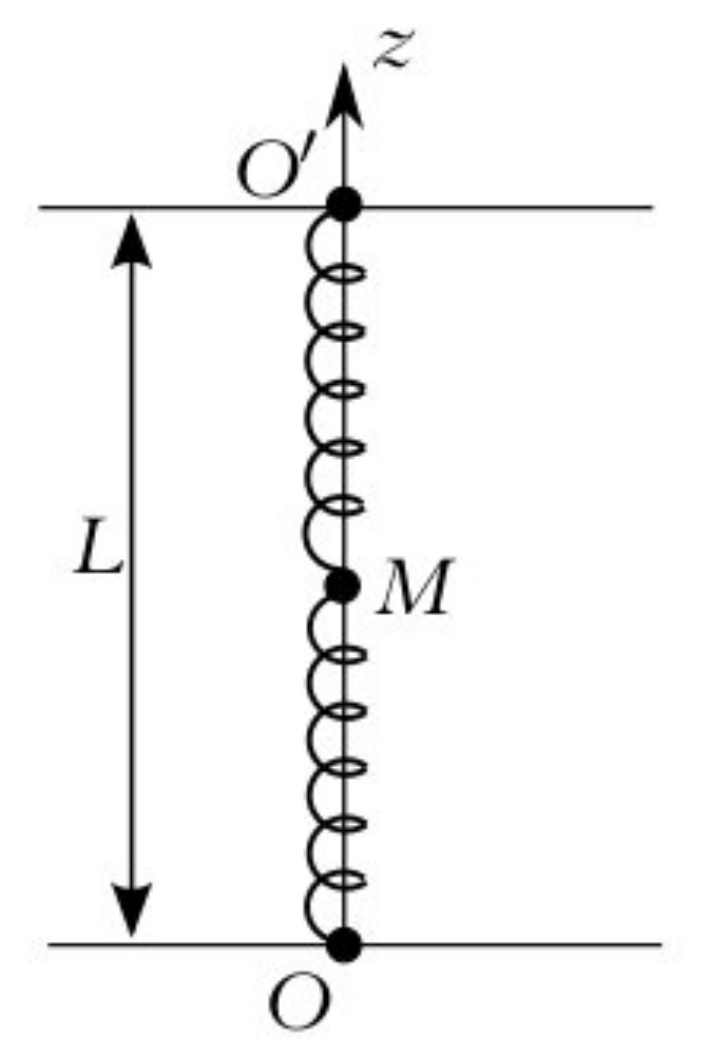
\includegraphics[width=\linewidth]{masse_2R-plain}
		\end{center}
	\end{minipage}
}

\QR{%
	Déterminer la position d'équilibre $z\ind{eq}$ de M.
}{%
	On étudie ici le point matériel M de masse $m$, dans le référentiel du
	laboratoire supposé galiléen avec le repère (O,$\uz$), $\uz$ vertical
	ascendant. On repère le point M par son altitude $\OMr = z(t)$.
	On effectue le \textbf{bilan des forces}~:
	\[
		\begin{array}{ll}
			\textbf{Poids}     & \Pf = m\gf = -mg\uz \\
			\textbf{Ressort 1} & \Ff\ind{ressort 1}
			= -k(\OMr - \ell_0)\uz = -k(z-\ell_0)\uz \\
			\textbf{Ressort 2} & \Ff\ind{ressort 2}
			= +k({\rm O'M} - \ell_0)\uz = +k(L-z-\ell_0)\uz
		\end{array}
	\]
	avec le ressort 1 celui d'en-dessous, le ressort 2 celui d'au-dessus. On
	notera simplement $\Ff_1$ et $\Ff_2$ dans la suite.
	Avec le PFD, on a
	\begin{gather*}
		m\af = \Pf + \Ff_1 + \Ff_2\\
		\Lra
		m\zpp = -mg -k(z - \cancel{\ell_0}) + k(L - z -\cancel{\ell_0})\\
		\Lra
		\boxed{\zpp + \frac{2k}{m}z = \frac{k}{m}L -g}
	\end{gather*}
	À l'équilibre, le ressort ne bouge plus~; on a donc $\zp = \zpp = 0$, et
	on trouve ainsi $z\ind{eq}$~:
	\[\boxed{z\ind{eq} = \frac{L}{2} - \frac{mg}{2k}}\]
	Sans la pesanteur, la masse sera à l'équilibre entre les deux ressorts,
	en toute logique. La gravité diminue cette altitude. On remarque que
	cette association de ressort est équivalente à avoir un seul ressort de
	raideur $2k$.
}

\QR{%
	Déterminer l'équation différentielle à laquelle satisfait $z(t)$.
	On écrira cette équation en fonction de $\w_0$ à définir et de
	$z\ind{eq}$.
}{%
	On a commencé la détermination de l'équation différentielle dans la
	question 2. On peut simplifier son expression en remarquant qu'à droite
	du signe égal, on doit trouver quelque chose homogène à $\w_0{}^2z$. On
	commence par identifier $\w_0$ avec la forme canonique~:
	\[\w_0 = \sqrt{\frac{2k}{m}}
		\qdonc
		\frac{k}{m}L - g = \w_0{}^2z\ind{eq}
	\]
	et finalement,
	\[\boxed{\zpp + \w_0{}^2z = \w_0{}^2z\ind{eq}}\]
}

\QR{%
	On écarte M d'une hauteur $a$ par rapport à sa position
	d'équilibre, et on le lâche sans vitesse. Déterminer $z(t)$.
}{%
	ion complète $z(t)$ et la somme de la solution particulière
	constante $z_p$ et de la solution homogène $z_h$. La solution
	particulière est, par définition, $z\ind{eq}$ (on l'a montré question 1).
	La solution homogène est celle d'un oscillateur harmonique, à savoir
	\[z_h = A\cos(\w_0t) + B\sin(\w_0t)\]
	Ainsi,
	\[z(t) = z\ind{eq} + A\cos(\w_0t) + B\sin(\w_0t)\]
	On trouve $A$ et $B$ avec les conditions initiales~:
	\begin{itemize}
		\item $z(0) = z\ind{eq} + a$ (masse lâchée d'une hauteur $a$ par
		      rapport à la position d'équilibre), or $z(0) = A + z\ind{eq}$,
		      donc
		      \[A = a\]
		\item $\zp(0) = 0$ (masse lâchée sans vitesse initiale), or $\zp(0)
			      = B\w_0$ donc
		      \[B = 0\]
	\end{itemize}
	\leftcenters{Ainsi,}{$\boxed{z(t) = z\ind{eq} + a\cos(\w_0t)}$}
}

\resetQ
\section{Plan incliné et frottements solides}

\enonce{%
	\noindent
	\begin{minipage}{0.6\linewidth}
		On considère un plan incliné d'un angle $\alpha = \ang{20;;}$ par rapport à
		l'horizontale. Une brique de masse $m = \SI{600}{g}$ est lancée depuis le
		bas du plan vers le haut, avec une vitesse $v_0 = \SI{2.4}{m.s^{-1}}$. Pour
		étudier le mouvement, on utilise le repère (O,$x$,$y$) avec O coïncidant
		avec la position de départ de la brique. On note $g$ l'accélération de la
		pesanteur, avec $g = \SI{9.81}{m.s^{-2}}$. \bigbreak
	\end{minipage}
	\hfill
	\begin{minipage}{0.35\linewidth}
		\begin{center}
			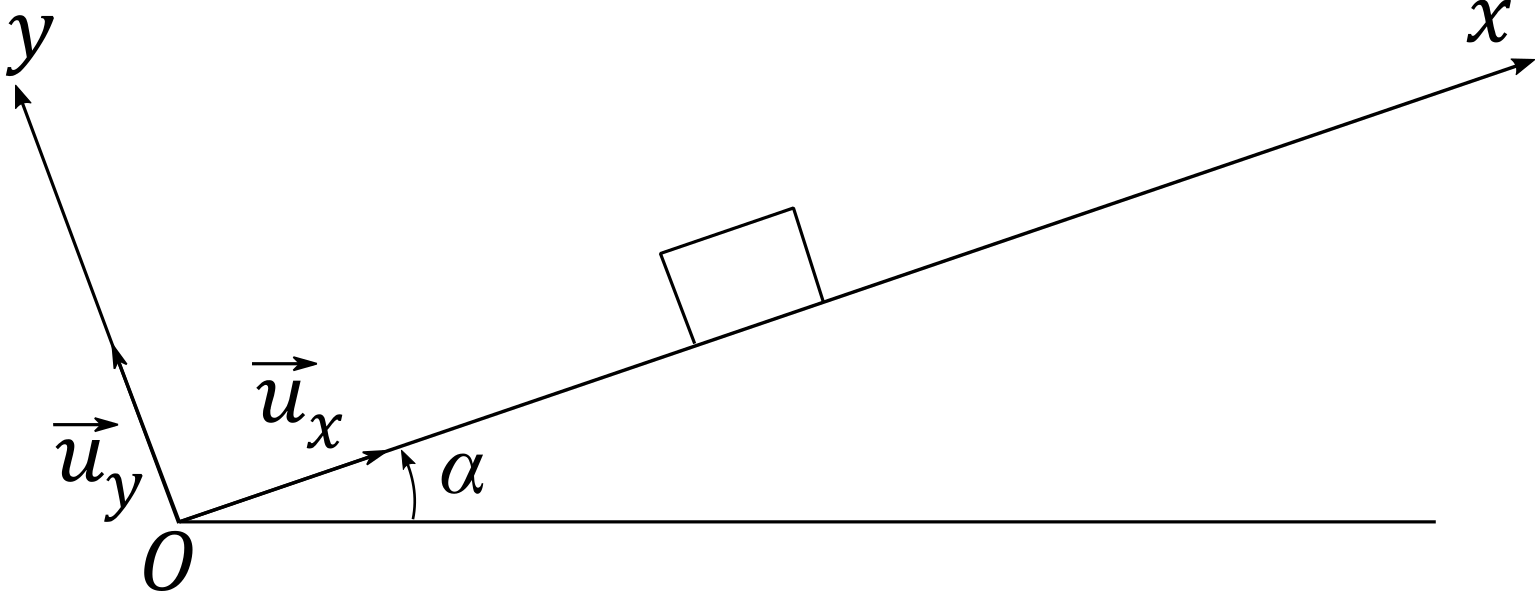
\includegraphics[width=\linewidth]{plan_incl-plain}
		\end{center}
	\end{minipage}
}

\begin{blocQR}
	\item On suppose en premier lieu que le contact entre la brique et le plan
	incliné se fait sans frottements
	\resetQ
	\QR{%
		Établir l'équation horaire du mouvement de la brique lors de
		sa montée.
	}{%
		\begin{itemize}
			\bitem{Système~:} \{brique\}
			\bitem{Référentiel~:} galiléen $(\Or, \ux, \uy)$ (voir schéma)
			\bitem{O et $t$ initial~:} tels que $\OM(0) = \of$
			\bitem{Vitesse initiale~:} $\vf(0) = v_0\ux$
			\bitem{Bilan des forces~:}
			\[
				\begin{array}{ll}
					\textbf{Poids}    & \Pf = -mg\cos\a\uy - mg\sin\a\ux \\
					\textbf{Réaction} & \Rf = R\uy
				\end{array}
			\]
			\bitem{PFD~:}
			\begin{gather*}
				m\af = \Pf + \Rf
				\Lra
				\left\{
				\begin{array}{rcl}
					\cancel{m}\xpp & = & -\cancel{m}g\sin\a \\
					\underbrace{\cancel{m\ypp}}_{=0}
					               & = & -mg\cos\a + R
				\end{array}
				\right.
			\end{gather*}
		\end{itemize}
		Il n'y a pas de mouvement sur $\uy$ étant donné que le mouvement
		se fait selon $\ux$~; ainsi $\boxed{y = \yp = \ypp = 0}$, et la
		seconde équation donne
		\[R = mg\cos\a\]
		On intègre la première pour avoir l'équation horaire sur $x(t)$~:
		\begin{gather*}
			\xp(t) = -gt\sin\a+v_0
			\Ra
			\boxed{x(t) = -\frac{1}{2}gt^2\sin\a + v_0t}
		\end{gather*}
		avec les conditions initiales $\xp(0) = v_0$ et $x(0) = 0$.
	}

	\QR{%
		Déterminer la date à laquelle la brique s'arrête, ainsi que la
		distance qu'elle aura parcourue.
	}{%
		On trouve le temps d'arrêt quand la vitesse est nulle. Soit
		$t_s$ ce temps d'arrêt~:
		\begin{gather*}
			\xp(t_s) = 0
			\Lra
			v_0 = gt_s\sin\a
			\Lra
			\boxed{t_s = \frac{v_0}{g\sin\a}}
		\end{gather*}
		On remarque alors que si $\a = 0$, $t_s \rightarrow +\infty$, ce
		qui est logique puisque sans frottement la brique ne
		s'arrêterait jamais. On obtient la distance d'arrêt en injectant
		ce temps dans $x(t)$~:
		\begin{gather*}
			x(t_s) = -\frac{1}{2}\cancel{g}
			\frac{v_0{}^2}{g^{\cancel{2}}\sin^{\bcancel{2}}\a}
			\bcancel{\sin\a} + v_0 \frac{v_0}{g\sin\a}
			\Lra
			\boxed{x(t_s) = \frac{1}{2}\frac{v_0{}^2}{g\sin\a}}
		\end{gather*}
	}

	\item On suppose ensuite qu'il existe des frottements solides, avec $f$ le
	coefficient de frottements solides tel que $f = \num{0.20}$.
	\resetQ
	\QR{%
		Établir l'équation horaire du mouvement de la brique lors de
		sa montée.
	}{%
		On reprend le même système, mais le bilan des forces change~:
		\begin{itemize}
			\bitem{Bilan des forces~:}
			\[
				\begin{array}{ll}
					\textbf{Poids}    & \Pf = -mg\cos\a\uy - mg\sin\a\ux \\
					\textbf{Réaction} & \Rf = R_N\uy -R_T\ux
				\end{array}
			\]
			En effet, sur la montée de la brique, sa vitesse est
			dirigée vers $+\ux$, donc la force de frottement (qui
			est une force de freinage et donc opposée à la vitesse)
			est dirigée vers $-\ux$. De plus, avec les lois du
			frottement de \textsc{Coulomb}, sur la montée la brique
			glisse sur le support, on a donc
			\[\boxed{R_T = fR_N}\]
			\bitem{PFD~:}
			\begin{gather*}
				m\af = \Pf + \Rf
				\Lra
				\left\{
				\begin{array}{rcl}
					m\xpp & = & -mg\sin\a - fR_N \\
					\underbrace{\cancel{m\ypp}}_{=0}
					      & = & -mg\cos\a + R_N
				\end{array}
				\right.
			\end{gather*}
		\end{itemize}
		Il n'y a pas de mouvement sur $\uy$ étant donné que le mouvement
		se fait selon $\ux$~; ainsi $\boxed{y = \yp = \ypp = 0}$, et la
		seconde équation donne
		\[R_N = mg\cos\a\]
		Que l'on réinjecte dans la première~:
		\[\xpp = -g\sin\a - fg\cos\a\]
		On intègre cette dernière pour avoir l'équation horaire sur $x(t)$~:
		\begin{gather*}
			\xp(t) = -g(\sin\a + f\cos\a)t+v_0
			\Ra
			\boxed{x(t) = -\frac{1}{2}g(\sin\a + f\cos\a)t^2 + v_0t}
		\end{gather*}
		avec les conditions initiales $\xp(0) = v_0$ et $x(0) = 0$. On
		retrouve le résultat précédent en posant $f=0$.
	}

	\QR{%
		Déterminer la date à laquelle la brique s'arrête, ainsi que la
		distance qu'elle aura parcourue.
	}{%
		On trouve le temps d'arrêt quand la vitesse est nulle. Soit
		$t_s$ ce temps d'arrêt~:
		\begin{gather*}
			\xp(t_s) = 0
			\Lra
			v_0 = gt_s(\sin\a + f\cos\a)
			\Lra
			\boxed{t_s = \frac{v_0}{g(\sin\a + f\cos\a)}}
		\end{gather*}
		Ce temps est plus \textbf{court} que sans frottements. On
		obtient la distance d'arrêt en injectant ce temps dans $x(t)$~:
		\begin{gather*}
			x(t_s) = -\frac{1}{2}\cancel{g(\sin\a + f\cos\a)}
			\frac{v_0{}^2}{\left(g(\sin\a + f\cos\a)\right)^{\cancel{2}}}
			+ v_0 \frac{v_0}{g(\sin\a + f\cos\a)}\\
			\Lra
			\boxed{x(t_s) = \frac{1}{2}\frac{v_0{}^2}{g(\sin\a + f\cos\a)}}
		\end{gather*}
	}

	\item On suppose finalement que la brique est \textbf{posée} sur le plan
	avec $\alpha$ variable.
	\resetQ
	\QR{%
		Quel doit être l'angle $\alpha$ pour que l'objet se mette en
		mouvement~?
	}{%
		Cette fois, la brique est initialement à l'arrêt, soit $\af(0)
			= \of$, et la brique ne glisse pas donc $R_T < fR_N$. On aura
		mouvement quand il y aura glissement, c'est-à-dire quand $R_T =
			fR_N$. On reprend donc le système précédent avec $\af = \of$~:
		\begin{gather*}
			\underbrace{\bcancel{m\af}}_{=\of} = \Pf + \Rf
			\Lra
			\left\{
			\begin{array}{rcl}
				0 & = & -mg\sin\a - fR_N \\
				0 & = & -mg\cos\a + R_N
			\end{array}
			\right.
			\Lra
			\left\{
			\begin{array}{rcl}
				\sin\a & = & f\cos\a  \\
				R_N    & = & mg\cos\a
			\end{array}
			\right.\\
			\Lra
			f = \tan\a
			\Lra
			\boxed{\alpha = \atan(f)}
		\end{gather*}
	}

	\QR{%
		Si le plan est en bois et la brique en métal, donner la valeur
		de cet angle. Même question si la brique est en bois. On donne
		\[
			f_{\text{fer/chêne}} = \num{0.26}
			\qet
			f_{\text{chêne/chêne}} = \num{0.34}
		\]
	}{%
		\leftcenters{On trouve}{
			$\boxed{\a\ind{fer/chêne} = \ang{14}}
				\qet
				\boxed{\a\ind{chêne/chêne} = \ang{19}}
			$}
	}

	\item Avec $\alpha = \ang{0;;}$, on souhaite déplacer une armoire de
	\SI{100}{kg} en tirant dessus avec la force $\Ff$. On donne
	$f_{\text{armoire/sol}} = \num{0.25}$.
	\resetQ
	\QR{%
		Déterminer la valeur de $\Ff$ pour mettre en mouvement
		l'armoire.
	}{%
		\begin{itemize}
			\bitem{Système~:} \{armoire\}
			\bitem{Référentiel~:} $(\Or, \ux, \uy)$ avec $\uy$ vertical
			asendant
			\bitem{Repère~:} On suppose la force de traction dirigée
			vers $+\ux$, et donc la vitesse de l'armoire selon $+\ux$
			\bitem{Repérage~:} $\OM = x(t)\ux$, $\vf = \xp(t)\ux$, $\af = \xpp(t)\ux$
			\bitem{Bilan des forces}~:
			\[
				\begin{array}{ll}
					\textbf{Poids}                 & \Pf = m\gf = -mg\uy \\
					\textbf{Réaction normale}      & \Rf_N = R_N\uy      \\
					\textbf{Réaction tangentielle} & \Rf_T =
					-R_T\ux                                              \\
					\textbf{Traction}              & \Ff = F\ux
				\end{array}
			\]
			À la limite du glissement, on a $R_T = fR_N$.
			\bitem{PDF~:} quand le mouvement est lancé, l'accélération est
			nulle.
			\begin{gather*}
				\underbrace{\bcancel{m\af}}_{=0}
				= \Pf + \Rf_N + \Rf_T + \Ff
				\Lra
				\left\{
				\begin{array}{rcl}
					0 & = & -mg + R_N \\
					0 & = & F - fR_N
				\end{array}
				\right.\\
				\Lra
				\left\{
				\begin{aligned}
					R_N       & = mg   \\
					\Aboxed{F & = fmg}
				\end{aligned}
				\right.
				\qavec
				\left\{
				\begin{array}{rcl}
					m & = & \SI{100}{kg}      \\
					g & = & \SI{10}{m.s^{-2}} \\
					f & = & \num{0.25}
				\end{array}
				\right.\\
				\AN
				\boxed{F = \SI{250}{N}}
				\Lra
				\boxed{\frac{F}{g} = \SI{25}{kg}}
			\end{gather*}
		\end{itemize}
		Ainsi, il suffit de fournir une force égale à un quart du poids.
	}

	\QR{%
		En déduire à quoi sert de mettre des patins en téflon sur les
		pieds de l'armoire.
	}{%
		Mettre des patins permet de diminuer le coefficient de
		frottement, et donc de diminuer la force de traction nécessaire
		pour déplacer le meuble.
	}
\end{blocQR}

% La réaction $\Rf$ du plan sur la brique s'exprime donc $\Rf = \Nf + \Tf$, avec
% $\Tf$ colinéaire de sens contraire au vecteur vitesse

\resetQ
\section{Coup franc et frottements fluides}

\enonce{%
	\noindent
	\begin{minipage}{0.45\linewidth}
		On étudie dans le référentiel terrestre galiléen de repère fixe (O,$x$,$y$),
		un coup franc de football tiré à \SI{20}{m}, face au but de hauteur
		\SI{2,44}{m} et dans son plan médian vertical ($x$O$y$). L'axe (O$y$) est
		choisi suivant la verticale ascendante.
	\end{minipage}
	\hfill
	\begin{minipage}{0.45\linewidth}
		\begin{center}
			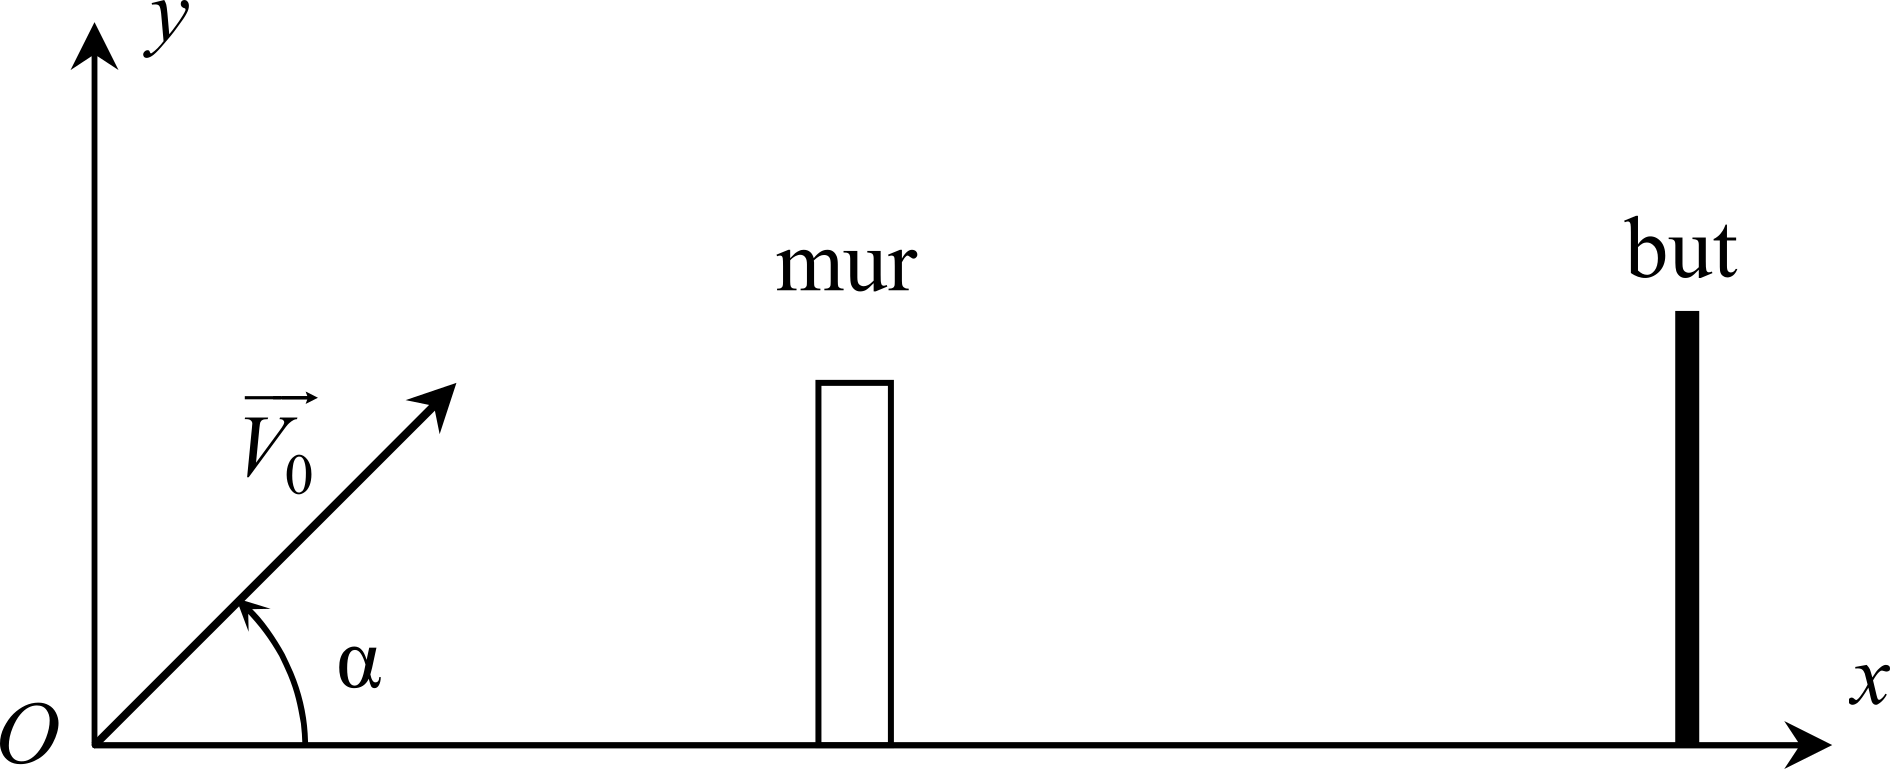
\includegraphics[width=\linewidth]{coup_franc-plain}
		\end{center}
	\end{minipage}
	\smallbreak
	Le ballon, de masse $m = \SI{430}{g}$, est assimilé à un point matériel M
	initialement au sol en O. Le mur, de hauteur \SI{1,90}{m}, est situé à
	\SI{9,15}{m} du ballon. Le ballon est lancé à l'instant $t = 0$ avec une vitesse
	initiale $v_0$ de norme \SI{20}{m.s^{-1}} et formant un angle $\alpha$ de
	\ang{20;;} avec l'horizontale. On note $g$ l'accélération de la pesanteur et on
	rappelle que $g = \SI{9,81}{m.s^{-2}}$.
}

\begin{blocQR}
	\item Dans un premier temps, on néglige totalement les frottements de l'air.
	\QR{%
		Établir les équations horaires du mouvement du ballon ainsi
		que l'équation de la trajectoire.
	}{%

		\begin{itemize}
			\bitem{Système~:} \{ballon\}
			\bitem{Référentiel~:} terrestre galiléen
			\bitem{Repère~:} cartésien $(\Or,\ux,\uy)$, $\uy$ vertical
			ascendant, $\ux$ vers le but
			\bitem{Repérage~:} $\OM = x(t)\ux + y(t)\uy$, $\vf = \xp(t)\ux +
				\yp(t)\uy$, $\af = \xpp(t)\ux + \ypp(t)\uy$
			\bitem{Origine et instant initial~:} $\OM(0) = \of$
			\bitem{Vitesse initiale~:} $\vf(0) = v_0\cos\a\ux +
				v_0\sin\a\uy$
			\bitem{BDF~:}
			\[
				\begin{array}{ll}
					\textbf{Poids} & \Pf = m\gf = -mg\uy
				\end{array}
			\]
			\bitem{PFD~:}
			\begin{gather}
				\label{eq:foot1pfd}
				\cancel{m}\af = -\cancel{m}g\uy
				\Lra
				\left\{
				\begin{array}{rcl}
					\xpp & = & 0  \\
					\ypp & = & -g
				\end{array}
				\right.
			\end{gather}
		\end{itemize}
		Ainsi,
		\begin{gather}
			\label{eq:foot1eqho}
			\eqref{eq:foot1pfd}
			\Ra
			\left\{
			\begin{array}{rcl}
				\xp & = & v_0\cos\a       \\
				\yp & = & -gt + v_0\sin\a
			\end{array}
			\right.
			\Ra
			\left\{
			\boxed{
				\begin{aligned}
					x(t) & = v_0t\cos\a                    \\
					y(t) & = -\frac{1}{2}gt^2 + v_0t\sin\a
				\end{aligned}
			}
			\right.
		\end{gather}
		étant donné les conditions initiales. On trouve la
		trajectoire en isolant $t(x)$ pour avoir $y(x)$~:
		\begin{gather*}
			\eqref{eq:foot1eqho}
			\Ra
			\left\{
			\begin{aligned}
				t(x) & = \frac{x}{v_0\cos\a}               \\
				\Aboxed{
				y(x) & = - \frac{g}{2v_0{}^2\cos^2\a}x^2 +
				x\tan\a}
			\end{aligned}
			\right.
		\end{gather*}
	}
	\QR{%
		Le ballon passe-t-il au-dessus du mur~?
	}{%
		Le ballon passe au-dessus du mur si $y(x\ind{mur}) \geq
			h\ind{mur}$ avec $h\ind{mur}$ la hauteur du mur et $x\ind{mur}$
		sa position horizontale. Avec une application numérique, on
		obtient
		\[y(x\ind{mur}) = \SI{2.17}{m} > h\ind{mur} = \SI{1.90}{m}\]
		donc le ballon \underline{passe bien au-dessus du mur}.
	}

	\QR{%
		Le tir est-il cadré~?
	}{%
		Le tir est cadré si $y(x\ind{but}) \leq h\ind{but}$. Or,
		\[y(x\ind{but}) = \SI{1.73}{m}\]
		donc \underline{le tir est bien cadré}.
	}

	\item Il y a en réalité des frottements, modélisés par une force $\Ff_f =
		-h\vf$ avec $h$ une constante positive de valeur
	$\SI{5.00e-3}{kg.s^{-1}}$.
	\resetQ
	\QR{%
		Déterminer les équations horaires en introduisant la constante
		$\tau = \frac{m}{h}$.
	}{%
		Avec le même système, seul le bilan des forces est modifié (et
		donc le PFD)~:
		\begin{itemize}
			\bitem{BDF~:}
			\[
				\begin{array}{ll}
					\textbf{Poids}       & \Pf = -mg\uy           \\
					\textbf{Frottements} & \Ff = -h\vf = -h\xp\ux
					-h\yp\uy
				\end{array}
			\]
			\item \leftcenters{\bfseries
				      PFD~:}{$m\af = -mg\uy -h\xp\ux -h\yp\uy$}
		\end{itemize}
		\vspace{-10pt}
		\begin{align*}
			\Lra
			\left\{
			\begin{aligned}
				m\xpp & = -h\xp     \\
				m\ypp & = -mg -h\yp
			\end{aligned}
			\right.
			 & \Lra
			\left\{
			\begin{aligned}
				\xpp + \frac{h}{m}\xp & = 0  \\
				\ypp + \frac{h}{m}\yp & = -g
			\end{aligned}
			\right.
			\\\Lra
			\left\{
			\begin{aligned}
				\dot{v_x} + \frac{v_x}{\tau} & = 0  \\
				\dot{v_y} + \frac{v_y}{\tau} & = -g
			\end{aligned}
			\right.
			 & \Lra
			\left\{
			\begin{aligned}
				v_x(t) & = A\exr^{-t/\tau}          \\
				v_y(t) & = -g\tau + B\exr^{-t/\tau}
			\end{aligned}
			\right.
			\\
			\text{Or,}\quad
			\left\{
			\begin{aligned}
				v_x(0) & = v_0\cos\a \\
				v_y(0) & = v_0\sin\a
			\end{aligned}
			\right.
			 & \Ra
			\left\{
			\begin{aligned}
				A & = v_0\cos\a         \\
				B & = v_0\sin\a + g\tau
			\end{aligned}
			\right. \\
			\text{donc}\quad
			\left\{
			\begin{aligned}
				v_x(t) & = v_0\cos\a\exr^{-t/\tau} \\
				v_y(t) & = \left(v_0\sin\a
				+ g\tau\right)\exr^{-t/\tau}
				-g\tau
			\end{aligned}
			\right.
			 & \Ra
			\left\{
			\begin{aligned}
				x(t) & = -v_0\tau\cos\a\exr^{-t/\tau}
				+ C                                   \\
				y(t) & = -\left(v_0\tau\sin\a
				+ g\tau^2\right)\exr^{-t/\tau}
				-g\tau t + D
			\end{aligned}
			\right. \\
			\qor
			\left\{
			\begin{aligned}
				x(0) & = 0 \\
				y(0) & = 0
			\end{aligned}
			\right.
			 & \Ra
			\left\{
			\begin{aligned}
				C & = v_0\tau\cos\a                         \\
				D & = -\left(v_0\tau\sin\a + g\tau^2\right)
			\end{aligned}
			\right.
		\end{align*}
		Finalement,
		\begin{empheq}[box=\fbox, left=\empheqlbrace]{align}
			\label{eq:foot2x}
			x(t) &= v_0\tau\cos\a\left(1 - \exr^{-t/\tau}\right)\\
			\label{eq:foot2y}
			y(t) &= \left(v_0\tau\sin\a + g\tau^2\right)
			\left(1-\exr^{-t/\tau}\right) -g\tau t
		\end{empheq}
	}
	\QR{%
		Donner l'équation de la trajectoire.
	}{%
		On isole $t(x)$ de \eqref{eq:foot2x} pour l'injecter dans
		\eqref{eq:foot2y}~:
		\begin{empheq}[box=\fbox, left=\empheqlbrace]{align*}
			% \label{eq:foot2t}
			t(x) &= -\tau\ln(1- \frac{x}{v_0\tau\cos\a})\\
			% \label{eq:foot2traj}
			y(x) &= \left(\tan\a + \frac{g\tau}{v_0\cos\a}\right)x
			+g\tau^2\ln(1- \frac{x}{v_0\tau\cos\a})
		\end{empheq}
	}
	\QR{%
		Le ballon passe-t-il au-dessus du mur~?
	}{%
		On calcule~:
		\[y(x\ind{mur}) = \SI{2.17}{m}\]
		donc \underline{le ballon passe au-dessus du mur}.
	}
	\QR{%
		Le tir est-il cadré~?
	}{%
		On calcule~:
		\[y(x\ind{but}) \approx \SI{1.73}{m}\]
		donc \underline{le tir est bien cadré}. On constate que les
		frottements n'ont eu que peu d'influence sur ce mouvement~; il
		n'est en effet pas très rapide, donc la force de frottements est
		restée assez faible.
	}
\end{blocQR}

\resetQ
\section{Charge soulevée par une grue}

\enonce{%
	Une grue de chantier de hauteur $h$ doit déplacer d'un point à un autre du
	chantier une charge M de masse $m$ supposée ponctuelle. On appelle A le point
	d'attache du câble sur le chariot de la grue.
	\smallbreak
	\noindent
	\begin{minipage}{0.45\linewidth}
		\begin{center}
			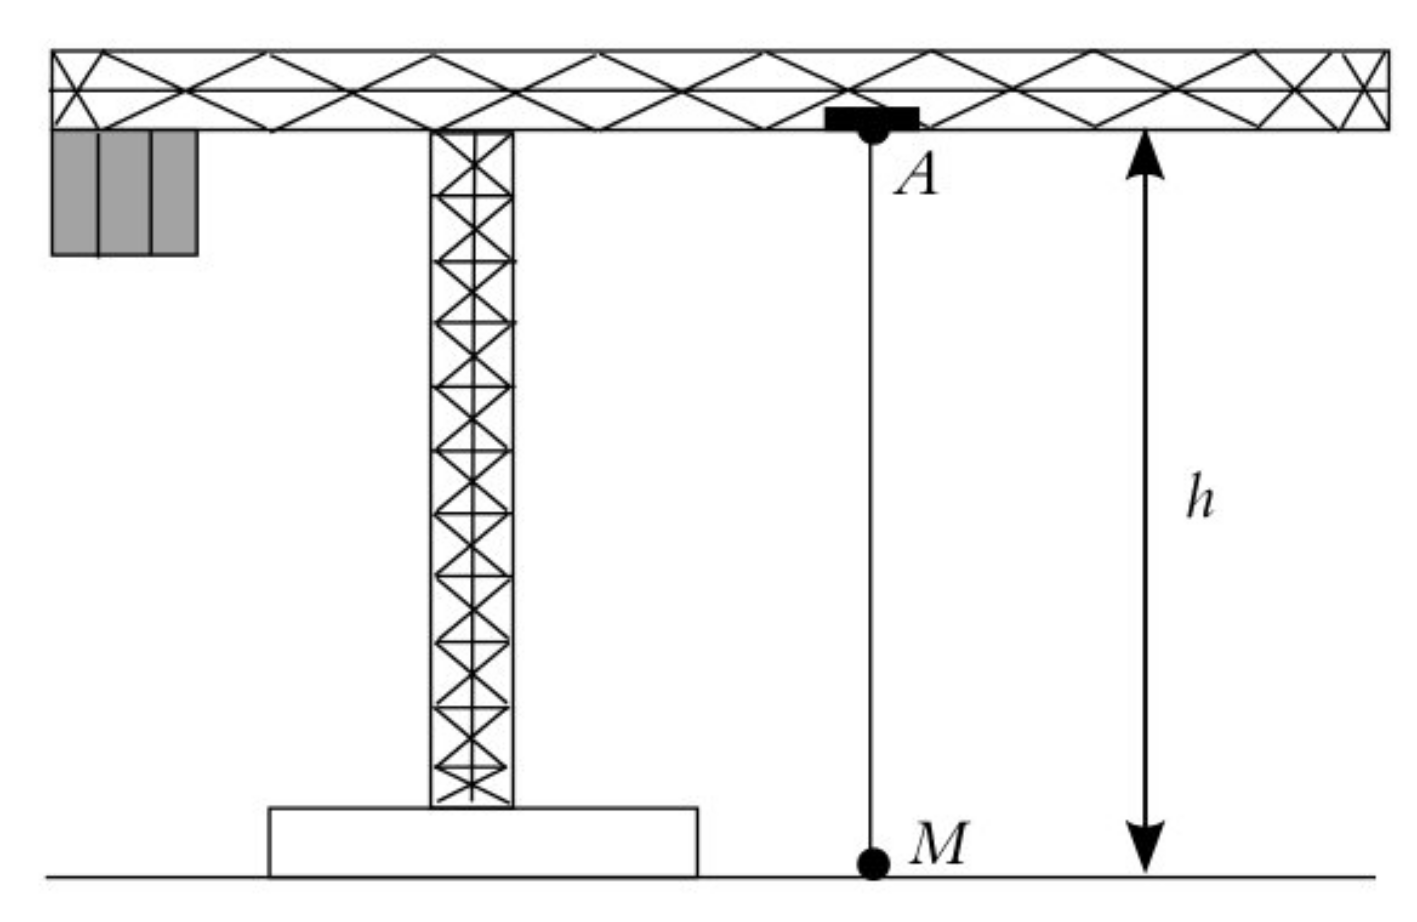
\includegraphics[height=3cm]{grue_fig1-plain}
			\captionof{figure}{Mouvement vertical}
			\label{fig:grue1_plain}
		\end{center}
	\end{minipage}
	\hfill
	\begin{minipage}{0.45\linewidth}
		\begin{center}
			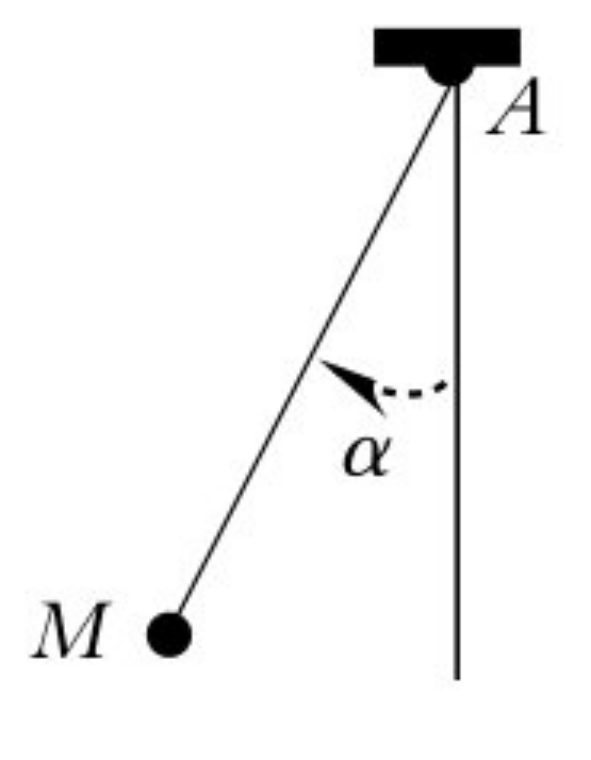
\includegraphics[height=3cm]{grue_fig2-plain}
			\captionof{figure}{Mouvement horizontal}
			\label{fig:grue2_plain}
		\end{center}
	\end{minipage}
}

\QR{%
	Le point A est à la verticale de M posée sur le sol. Déterminer la
	tension du câble lorsque M décolle (figure~\ref{fig:grue1_plain}).
}{%
	\begin{itemize}
		\bitem{Système~:} \{masse $m$\} repérée par son centre d'inertie $M$.
		\bitem{Référentiel~:} relié au sol, galiléen.
		\bitem{Coordonnées~:} cartésiennes, $(\Or,\ux,\uy,\uz)$ avec $\uz$
		vertical ascendant, O au pieds de la grue.
		\bitem{BDF~:} avant qu'elle ne décolle, il y a la réaction du sol~; on
		s'intéresse au décollage, donc au moment où elle s'annule. On
		aura donc
		\[
			\begin{array}{ll}
				\textbf{Poids}   & \Pf = m\gf = -mg\uz \\
				\textbf{Tension} & \Tf = T\uz
			\end{array}
		\]

		\bitem{PFD~:} au moment où la masse décolle, son accélération est
		positive et selon $\uz$, soit $\af = \zpp\uz$~; en supposant un
		décollage en douceur, $\zpp \approx 0$, soit
		\[
			m\af = \Pf + \Tf
			\Lra
			0 = -mg + T
			\Lra
			\boxed{T = mg}
		\]
		On a donc la tension égale au poids.
	\end{itemize}
}
\QR{%
	L'enrouleur de câble de la grue remonte le câble avec une accélération
	$a_v$ constante. Déterminer la tension du câble et conclure.
}{%
	\leftcenters{Dans ce cas, on a explicitement}{$\boxed{T = m(a_v+g)}$}
	\smallbreak
	La tension est supérieure au poids, et fonction affine de $a_v$~: si
	l'accélération est trop forte, le câble peut rompre.
}
\noindent
\begin{blocQR}
	\item La montée de M est stoppée à mi-hauteur mais le chariot A se met en
	mouvement vers la droite (figure~\ref{fig:grue2_plain}) avec une
	accélération $a_h$ constante.
	\QR{%
		Quelle est l'accélération de M sachant que M est alors immobile par
		rapport à A~?
	}{%
		L'accélération de M est $\af_M = \dv[2]{\OM}{t}$. Or, $\OM = \vv{\rm OA} +
			\vv{\rm AM}$ avec $\vv{\rm AM}$ constant~: ainsi
		\[\boxed{\af_M = \dv[2]{\OM}{t} = \dv[2]{\vv{\rm OA}}{t} =
				\af_h}\]
	}
	\QR{%
		Déterminer l'angle $\alpha$ (figure~\ref{fig:grue2_plain}) que fait le câble avec
		la verticale en fonction de $m$, $g$, $a_h$ ainsi que la tension
		du câble.
	}{%
		\noindent
		\begin{minipage}{.80\linewidth}
			On a alors le PFD~:
			\[
				m\af_h = m\gf + \Tf
				\Lra
				ma_h\ux = -mg\uz + T\cos\a\uz + T\sin\a\ux
			\]
			\leftcenters{Ainsi,}{
				$\DS \left\{
					\begin{aligned}
						ma_h & = T\sin\a \\
						mg   & = T\cos\a
					\end{aligned}
					\right.
					\Lra
					\boxed{
						\left\{
						\begin{aligned}
							\tan\a & = \frac{a_h}{g}         \\
							T      & = m\sqrt{a_h{}^2 + g^2}
						\end{aligned}
						\right.}$}
		\end{minipage}
		\hfill
		\begin{minipage}{0.15\linewidth}
			\begin{center}
				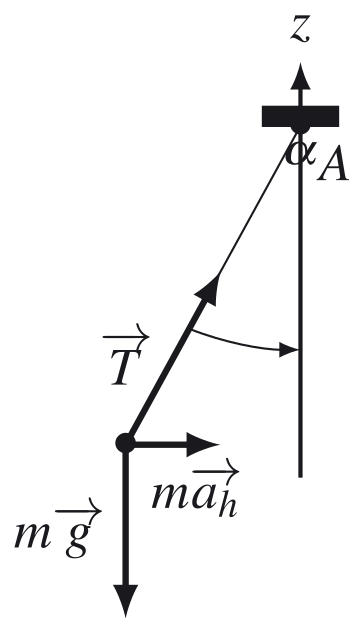
\includegraphics[width=\linewidth]{grue_corr}
			\end{center}
		\end{minipage}
	}
\end{blocQR}

\resetQ
\section{Étude d'un volant de badminton}

\enonce{%
	Un volant de badminton a une masse $m = \SI{5,0}{g}$. On veut vérifier
	expérimentalement l'information trouvée sur internet qui précise qu'un volant
	lâché de très haut atteint une vitesse limite $v_l = \SI{25}{km.h^{-1}}$. Pour
	tester cette affirmation, on veut déterminer l'altitude $h$ à laquelle il faut
	le lâcher (sans vitesse initiale) pour qu'il atteigne cette vitesse limite.
	\bigbreak
	On lâche le volant d'une fenêtre en hauteur et on filme sa chute verticale. On
	note O le point de départ de la chute, et (O$z$) l'axe vertical dirigé vers le
	bas. Au cours de la chute, on prend en compte une force de frottement due à
	l'air de la forme $\Ff = -\lambda v\vf$ où $\vf$ est le vecteur vitesse du point
	M, $v$ sa norme et $\lambda$ un coefficient positif. On note $g$ l'accélération
	de la pesanteur et on rappelle que $g = \SI{9,81}{m.s^{-2}}$.
}

\QR{%
	Établir l'équation différentielle portant sur la norme du vecteur
	vitesse $v(t)$.
}{%
	\begin{itemize}
		\bitem{Système~:} \{volant\} assimilé à un point matériel M de masse
		$m$
		\bitem{Référentiel~:} terrestre supposé galiléen
		\bitem{Repère~:} $(\Or, \uz)$ avec O départ de chute, $\uz$ vertical
		\textit{descendant} (voir schéma)
		\bitem{Repérage~:} $\OM = z(t)\uz$, $\vf = \zp(t)\uz$, $\af =
			\zpp(t)\uz$
		\bitem{Origine et instant initial~:} $\OM(0) = z(0)\uz = \of$
	\end{itemize}\smallbreak
	\begin{minipage}{0.70\linewidth}
		\begin{itemize}
			\bitem{BFD~:}
			\[
				\begin{array}{ll}
					\textbf{Poids}       & \Pf = m\gf = mg\uz    \\
					\textbf{Frottements} & \Ff = -\lambda v\vf =
					-\lb\zp^2\uz
				\end{array}
			\]
			\bitem{PFD~:}
			\[m\af = \Pf + \Ff \Lra m\zpp = mg -\lb\zp^2 \Lra \zpp +
				\frac{\lb}{m}\zp^2 = g\]
		\end{itemize}
	\end{minipage}
	\begin{minipage}{0.25\linewidth}
		\hfill
		\begin{center}
			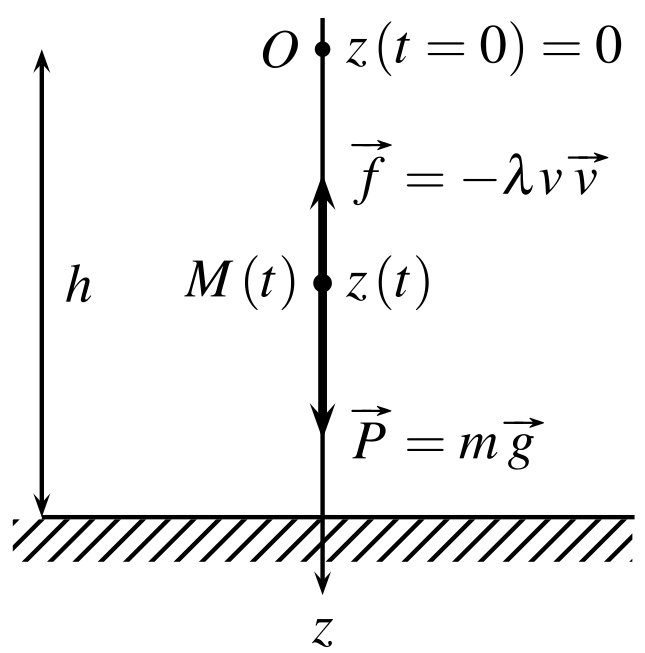
\includegraphics[width=\linewidth]{volant_corr}
		\end{center}
		\vspace{-30pt}
		\hfill~
	\end{minipage}\smallbreak
	\leftcenters{Ainsi,}{$\DS\boxed{\dv{v}{t} + \frac{\lb}{m}v^2 = g}$}
}

\QR{%
Montrer l'existence d'une vitesse limite $v_l$ et l'exprimer en
fonction de $\lambda$, $m$ et $g$.
}{%
Lorsqu'on lâche M sans vitesse initiale d'une hauteur $h$, la vitesse
est faible au départ et la force principale est le poids, accélérant le
mobile vers le bas. Quand la vitesse augmente, les frottements
s'intensifient jusqu'à ce qu'ils compensent le poids, donnant $\af =
	\of$~: la vitesse n'évolue plus et reste à sa valeur avant compensation,
la vitesse limite $v_l$. $v_l$ étant constante, $\vp_l = 0$, donc
l'équation différentielle donne
\[
	\frac{\lb}{m}v_l{}^2 = g
	\Lra
	\boxed{v_l = \sqrt{\frac{mg}{\lb}}}
\]
}

\enonce{%
	On note $t^* = t/\tau$, $z^* = z/L$ et $v^* = v/v_l$, avec $\tau = v_l/g$ et $L
		= v_l\tau$.
}

\QR{%
	Montrer que $t^*$, $z^*$ et $v^*$ sont trois grandeurs sans dimension.
}{%
	$v^*$ est le rapport de deux vitesses, donc est forcément sans
	dimension. Ensuite,
	\begin{gather*}
		[\tau] = \left[\frac{v_l}{g}\right] =
		\frac{\si{m.s^{-1}}}{\si{m.s^{-2}}} = \si{s}
		\\
		[L] = [v_l][\tau] = \si{m.s^{-1}}\times\si{s} = \si{m}
	\end{gather*}
	donc $\tau$ est bien un temps et $L$ une longueur~; ce faisant, $t^*$ et
	$z^*$ sont évidemment adimensionnées.
}

\QR{%
	Montrer que l'équation différentielle portant sur la vitesse peut se
	mettre sous la forme~:
	\[\dv{v^*}{t^*} + (v^*)^2 = 1\]
}{%
	On réécrit l'équation avec $v = v_lv^*$ et $t=\tau t^*$~:
	\begin{gather*}
		\dv{v}{t} + \frac{\lb}{m}v = g
		\Lra
		\dv{(v_lv^*)}{(\tau t^*)} + \frac{\lb}{m} \left(v_lv^*\right)^2 = g
		\Lra
		\frac{v_l}{\tau} \dv{v^*}{t^*} + \frac{\lb v_l{}^2}{m}(v^*)^2 = g
	\end{gather*}
	Or,
	\begin{gather*}
		\frac{v_l}{\tau} = g
		\qet
		\frac{\lb v_l{}^2}{m} = g
		\LRa
		\boxed{\dv{v^*}{t^*} + (v^*)^2 = 1}
	\end{gather*}
}
\enonce{%
	La résolution de l'équation précédente conduit à des solutions dont on donne les
	représentations graphiques ci-dessous.

	\begin{center}
		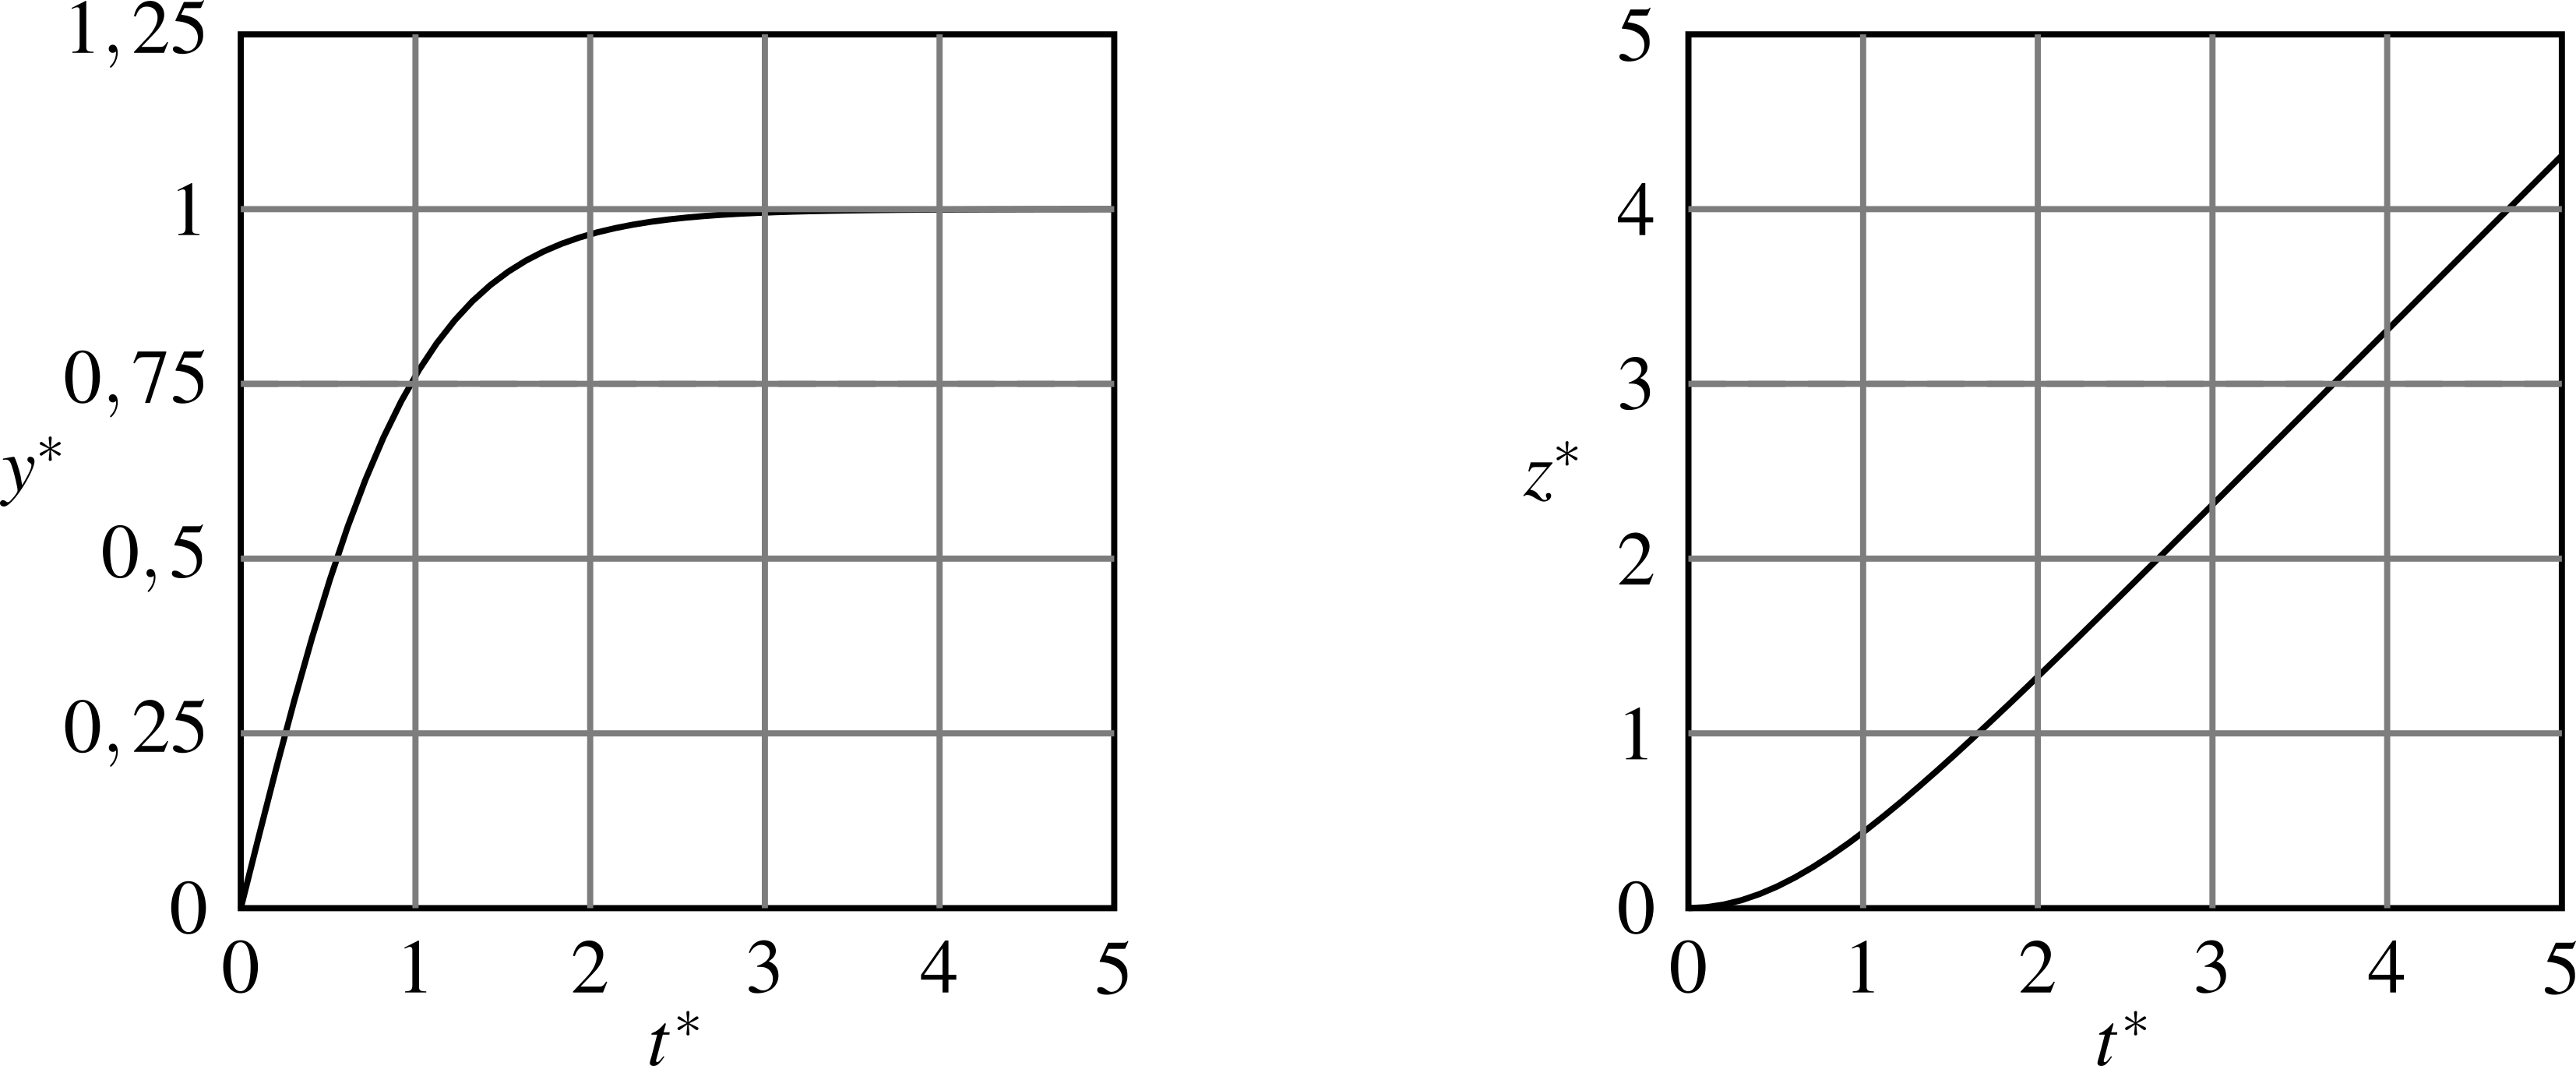
\includegraphics[width=.8\linewidth]{volant_data-plain}
	\end{center}
}

\QR{%
	À l'aide des courbes, décrire les deux phases du mouvement.
}{%
	Ces courbes montrent que la vitesse augmente pendant 2 à 3$\tau$,
	avant de se stabiliser à $v_l$. Le mouvement est ensuite rectiligne
	uniforme, et $z$ est une fonction affine du temps.
}
\QR{%
	Déterminer l'altitude minimale $h$ à laquelle il faut lâcher le volant
	pour que sa vitesse au sol soit supérieure ou égale à 95\% de $v_l$. On
	exprimera cette altitude en fonction de $L$. Déterminer également la
	durée $\D t$ de l'expérience en fonction de $\tau$.
}{%
	Le courbe représentant $v^*(t^*)$ montre que $v^* = \num{0.95}$ pour
	$t^* = \num{1.8}$. La durée de l'expérience pour arriver à cette valeur
	est donc $\SI{1.8}{\tau}$, et la hauteur $z^*$ à ce temps est $z^* =
		\num{1.2}$, ce qui correspond à $z = \SI{1.2}{L}$~; ainsi
	\[
		\boxed{\Dt = \SI{1.8}{\tau}}
		\qet
		\boxed{h = \SI{1.2}{L}}
	\]
}
\QR{%
	En admettant que la vitesse limite est proche de la valeur trouvée sur
	internet, calculer numériquement $L$ et $\tau$ puis $h$ et $\Dt$.
}{%
	En supposant $v_l$ connue, on a
	\begin{gather*}
		\tau = \frac{v_l}{g}
		\qet
		L = v_l\tau
		\qavec
		\left\{
		\begin{array}{rcl}
			v_l & = & \SI{25}{km.h^{-1}} = \SI{7.0}{m.s^{-1}} \\
			g   & = & \SI{9.81}{m.s^{-2}}
		\end{array}
		\right.\\
		\AN
		\boxed{\tau = \SI{7.1e-1}{s}}
		\qet
		\boxed{L = \SI{4.9}{m}}
	\end{gather*}
	Ainsi, \vspace*{-24pt}
	\begin{gather*}
		\Dt = \SI{1.8}{\tau}
		\qet
		h = \SI{1.2}{L}
		\\\Ra
		\boxed{\Dt = \SI{1.3}{s}}
		\qet
		\boxed{h = \SI{5.9}{m}}
	\end{gather*}
}

\resetQ
\section{Étude d'une skieuse}
\enonce{%
	On étudie le mouvement d'une skieuse descendant une piste selon la ligne de plus
	grande pente, faisant un angle $\alpha$ avec l'horizontale. L'air exerce une
	force de frottements supposée de la forme $\Ff = -\lambda\vf$ avec $\lambda$ un
	coefficient positif et $\vf$ le vecteur vitesse du skieur. \bigbreak
	On note $\Tf$ et $\Nf$ les composantes tangentielle et normale de la force de
	frottements exercée par la neige, et $f$ le coefficient de frottements solides
	tel que $\norm{\Tf} = f\norm{\Nf}$. \bigbreak
	On choisit comme origine de l'axe (O$x$) de la ligne le plus grande pente la
	position initiale de la skieuse, supposée partir à l'instant initiale avec une
	vitesse négligeable. On note (O$y$) l'axe normal à la piste en O et dirigée vers
	le haut.
}

\QR{%
	Calculer $\Tf$ et $\Nf$.
}{%
	\begin{minipage}[t]{0.60\linewidth}
		\begin{itemize}
			\bitem{Système~:} \{skieuse\} assimilée à son centre de gravité
			\bitem{Référentiel~:} $\Rc\ind{sol}$ supposé galiléen
			\bitem{Repère~:} $(\Or, \ux, \uy)$ (voir schéma)
			\bitem{Repérage~:} $\OM = x(t)\ux$~; $\vf = \xp(t)\ux$~; $\af =
				\xpp(t)\ux$.
			\bitem{Origine et instant initial~:} $\OM(0) = \of$
			\bitem{Vitesse initiale~:} $\vf(0) = \of$
		\end{itemize}
	\end{minipage}
	\hfill
	\begin{minipage}{0.35\linewidth}
		\begin{center}
			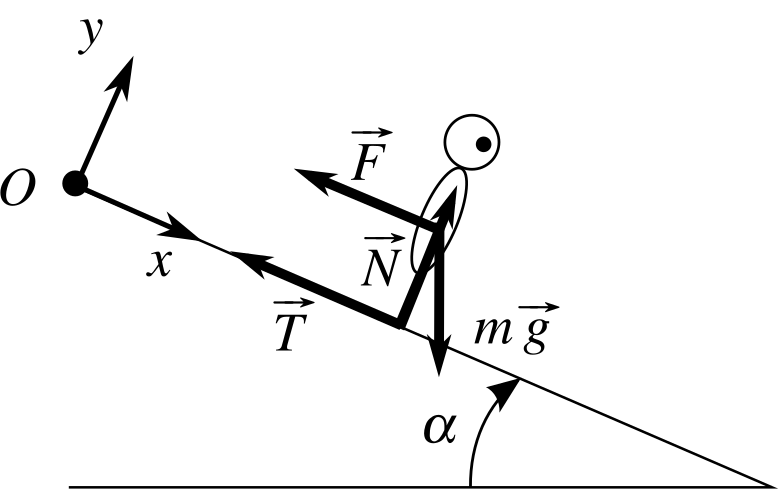
\includegraphics[width=.9\linewidth]{ski_corr}
		\end{center}
		\vspace{-3cm}
	\end{minipage}\smallbreak
	\begin{itemize}
		\bitem{BDF~:}
		\[
			\begin{array}{ll}
				\textbf{Poids}                 & m\gf = mg(\sin\a\ux - \cos\a\uy) \\
				\textbf{Réaction normale}      & \Nf = N\uy                       \\
				\textbf{Réaction tangentielle} & \Tf = -T\ux =
				-fN\ux                                                            \\
				\textbf{Frottements}           & \Ff = -\lb\vf = -\lb\xp\ux
			\end{array}
		\]
		Comme la skieuse glisse sur la piste, avec les lois du
		frottement de \textsc{Coulomb}, on a
		\[T = fN\]
		\bitem{PFD~:}
		\[
			m\af = \Pf + \Nf + \Tf + \Ff
			\Lra
			\left\{
			\begin{aligned}
				m\xpp & = mg\sin\a - fN - \lb\xp \\
				m\ypp & = -mg\cos\a + N
			\end{aligned}
			\right.
		\]
	\end{itemize}
	Ainsi, comme il n'y a pas de mouvement sur $\uy$, $\ypp = 0$ et
	\[
		\boxed{N = mg\cos\a}
		\Ra
		\boxed{T = fN = fmg\cos\a}
	\]
}
\QR{%
	Calculer la vitesse $\vf(t)$ et la position $x(t)$ de la skieuse à
	chaque instant $t$.
}{%
	On réutilise la première équation en y injectant l'expression de $T$
	pour avoir~:
	\[
		\xpp + \frac{\lb}{m}\xp = g(\sin\a - f\cos\a)
	\]
	Avec $\vf = \xp(t)\ux$, on obtient une équation différentielle sur
	$v(t)$ que l'on résout en posant $\tau = m/\lb$ avec la solution
	homogène $A\exr^{-t/\tau}$ et la solution particulière $v_p$~:
	\[
		\vp(t) + \frac{v}{\tau} = g(\sin\a - f\cos\a)
		\Ra
		v = A\exr^{-t/\tau} + v_p
	\]
	et on trouve $v_p$ directement en remarquant que, par construction,
	$\vp_p = 0$ donc $v_p = g\tau(\sin\a - f\cos\a)$. En combinant on peut
	utiliser la condition initiale sur la vitesse~:
	\begin{gather*}
		v(t) = A\exr^{-t/\tau} + g\tau(\sin\a - f\cos\a)
		\shortintertext{Or,}
		\left.
		\begin{aligned}
			v(0) & = 0
			\\\Lra
			0    & = A + g\tau(\sin\a - f\cos\a)
			\\\Lra
			A    & = -g\tau(\sin\a - f\cos\a)
		\end{aligned}
		\right\}
		\quad\Ra\quad
		\boxed{v(t) = g\tau(\sin\a - f\cos\a)\left(1-\exr^{-t/\tau}\right)}
	\end{gather*}
	On trouve la position $x(t)$ en intégrant $v(t)$~:
	\begin{gather*}
		x(t) = g\tau(\sin\a - f\cos\a)\left(t + \tau\exr^{-t/\tau}\right) +
		B
		\shortintertext{Or,}
		\left.
		\begin{aligned}
			x(0) & = 0
			\\\Lra
			0    & = g\tau(\sin\a - f\cos\a)\left(0 + \tau\right) + B
			\\\Lra
			B    & = -g\tau^2(\sin\a - f\cos\a)
		\end{aligned}
		\right\}
		\quad\Ra\quad
		\boxed{x(t) =
			g\tau(\sin\a-f\cos\a)\left(t+\tau\left(\exr^{-t/\tau}-1\right)\right)}
	\end{gather*}
}
\QR{%
	Montrer que la skieuse atteint une vitesse limite $\vf_l$ et exprimer
	$\vf(t)$ et $\OM(t)$ en fonction de $\vf_l$.
}{%
	La vitesse limite est la solution particulière $v_p$~:
	\[\boxed{\vf_l = g\tau(\sin\a-f\cos\a)\ux}\]
	En effet, la présence de la force de frottements fluides dont la norme
	augmente avec la vitesse fait que la vitesse ne peut pas augmenter
	indéfiniment. La skieuse atteint une vitesse limite lorsque les
	frottement compensent la force motrice du mouvement. Ainsi,
	\[
		\boxed{\vf(t) = v_l\left(1-\exr^{-t/\tau}\right)\ux}
		\qet
		\boxed{\OM(t) =
			v_l\left(t+\tau\left(\exr^{-t/\tau}-1\right)\right)\ux}
	\]
}
\QR{%
	Calculer $v_l = \norm{\vf_l}$ pour $\lambda = \SI{1}{kg.s^{-1}}$, $f =
		\num{0.9}$, $g = \SI{10}{m.s^{-1}}$, $m = \SI{65}{kg}$ et $\alpha =
		\ang{45;;}$.
}{%
	\begin{gather*}
		\boxed{v_l = \frac{mg}{\lb}(\sin\a-f\cos\a)}
		\qavec
		\left\{
		\begin{array}{rcl}
			m   & = & \SI{65}{kg}       \\
			g   & = & \SI{10}{m.s^{-2}} \\
			\lb & = & \SI{1}{kg.s^{-1}} \\
			\a  & = & \ang{45}          \\
			f   & = & \num{0.9}
		\end{array}
		\right.\\
		\AN
		\boxed{v_l = \SI{46}{m.s^{-1}}}
	\end{gather*}
	On remarque que la vitesse limite est une fonction affine du poids.
	Ainsi, le manque de représentation des femmes dans les sports d'hiver,
	souvent justifié par une moins bonne performance pure, est biaisé par la
	répartition moyenne de leurs tailles (et donc de leurs poids) plus
	faible que la répartition moyenne des tailles (et donc poids) des
	hommes, rendant \underline{pour certains} leurs records moins
	impressionnants.
}
\QR{%
	Calculer littéralement et numériquement la date $t_1$ où la skieuse a
	une vitesse égale à $v_l/2$.
}{%
	\begin{gather*}
		\begin{aligned}
			v(t_1)                 & = \frac{v_l}{2}
			\\\Lra
			\frac{\cancel{v_l}}{2} & = \cancel{v_l}(1-\exr^{-t_t/\tau})
			\\\Lra
			\frac{1}{2}            & = 1-\exr^{-t_1/\tau}
			\\\Lra
			\exr^{-t_1/\tau}       & = \frac{1}{2}
		\end{aligned}
		\\\Lra
		\boxed{t_1 = \tau\ln2}
		\qavec
		\tau = \frac{m}{\lb}
		\qet
		\left\{
		\begin{array}{rcl}
			m   & = & \SI{65}{kg}       \\
			\lb & = & \SI{1}{kg.s^{-1}}
		\end{array}
		\right.\\
		\AN
		\boxed{t_1 = \SI{45}{s}}
	\end{gather*}
}
\QR{%
	À la date $t_1$, la skieuse chute. On néglige alors la résistance de
	l'air et on considère que le coefficient de frottements sur le sol est
	multiplié par 10. Calculer la distance parcourue par la skieuse avant
	qu'elle ne s'arrête.
}{%
	En tombant à $t=t_1$, la skieuse a pour vitesse $v_l/2$. L'équation du
	mouvement sur $\uy$ ne change pas de forme, mais on multiplie $f$ par
	10, donc $T=10fmg$. Ainsi, en posant $t'=t-t_1$, en projection sur $\ux$
	et en négligeant $\lb$,
	\begin{gather*}
		\xpp(t') = g(\sin\a-10f\cos\a)
		\Ra
		\xp(t') = gt'(\sin\a-10f\cos\a) + v_l/2
	\end{gather*}
	On trouve le temps d'arrêt $t'_a$ quand $\xp(t'_a) = 0$, soit
	\[t'_a = \frac{-v_l}{2g(\sin\a-10f\cos\a)}\]
	et la distance d'arrêt depuis le point de chute en intégrant $\xp(t')$
	puis en prenant $x(t'_a)$~:
	\begin{gather*}
		x(t') = \frac{1}{2}gt'^2(\sin\a-10f\cos\a) + \frac{v_lt'}{2}
		\\\Lra
		\boxed{x(t'_a) = - \frac{v_l{}^2}{8g(\sin\a-10f\cos\a)}}
		\qavec
		\left\{
		\begin{array}{rcl}
			v_l & = & \SI{46}{m.s^{-1}} \\
			g   & = & \SI{10}{m.s^{-1}} \\
			\a  & = & \ang{45}          \\
			f   & = & \num{0.9}
		\end{array}
		\right.\\
		\AN
		\boxed{x(t'_a) = \SI{4.7}{m}}
	\end{gather*}
}

\end{document}
